%%
%% GMU LaTeX PhD Dissertation Format Template
%%
%% Developed by:
%%      Daniel O. Awduche and Christopher A. St. Jean
%%      Communications and Networking Lab
%%      Dept. of Electrical and Computer Engineering
%%
%% Notes on usage can be found in the accompanying USAGE_NOTES.txt file.
%%
%%**********************************************************************
%% Legal Notice:
%% This code is offered as-is without any warranty either
%% expressed or implied; without even the implied warranty of
%% MERCHANTABILITY or FITNESS FOR A PARTICULAR PURPOSE!
%% User assumes all risk.
%% In no event shall any contributor to this code be liable for any damages
%% or losses, including, but not limited to, incidental, consequential, or
%% any other damages, resulting from the use or misuse of any information
%% contained here.
%%**********************************************************************
%%
%% $Id: GMU_dissertation_template.tex,v 1.7 2007/05/02 02:20:38 Owner Exp $
%%

\documentclass[11 pt]{report}

%%  The file ``gmudissertation.sty''  is the GMU latex style file and
%%   should be placed in the same directory as your LaTeX files
\usepackage{gmudissertation}

%%
%% other packages that need to be loaded
%%
\usepackage{graphicx}                    %   for imported graphics
\usepackage{amsmath}                     %%
\usepackage{amsfonts}                    %%  for AMS mathematics
\usepackage{amssymb}                     %%
\usepackage{amsthm}                      %%
\usepackage[normalem]{ulem}              %   a nice standard underline package
\usepackage[noadjust,verbose,sort]{cite} %   arranges reference citations neatly
\usepackage{setspace}                    %   for line spacing commands
\usepackage{url}
\usepackage{notoccite} %So citations don't start in t.o.c. or figure list

%% The file ``mydissertationabbrev.sty'' is an (optional) personalized file that
%% may contain any and all LaTeX command (re)definitions that will be used
%% throughout the document
%\usepackage{mydissertationabbrev}

\beforedoc

\begin{document}

%% In this section, all of the user-specific fields to be used in the
%% title pages are set
\title{Statistical Modelling of Earth's plasmasphere}
\onelinetitle{Statistical Modelling of Earth's plasmasphere}
\author{Victoir Veibell}
\degree{Doctor of Philosophy}
\doctype{Dissertation}
\dept{Department of Computational and Data Sciences}
\discipline{Computational Space Sciences and Astrophysics}

\seconddeg{Master of Science}
\seconddegschool{George Mason University}
\seconddegyear{2014}

\firstdeg{Bachelor of Science}
\firstdegschool{Embry Riddle Aeronautical University}
\firstdegyear{2010}

\degreeyear{2016}

% Note: semester name should be written in its full-form. For example, Fall Semester, not just Fall.
\degreesemester{Spring Semester}

\advisor{Robert Weigel}

\firstmember{Kirk Borne}

\secondmember{Fernando Camelli}

\thirdmember{Jie Zhang}

\depthead{Maria Dworzecka}

% The current dean is Lloyd J. Griffiths
\deanITE{Peggy Agouris}

%%
%% Introductory pages
%%

% Note: The signature sheet is set according to the requirements of the Volgenau School of
% Information Technology and Engineering. If your college/school requirement is different,
% please make appropriate changes in the "signaturepage" section of gmudissertation.sty file.
\signaturepage

\titlepage

% copyright technically optional but should be included in to avoid potential pagination problems
\copyrightpage

%%
%% Dedication page
%%

\dedicationpage

\noindent I dedicate this dissertation to ...
I dedicate this dissertation to ...
I dedicate this dissertation to ...
I dedicate this dissertation to ...
I dedicate this dissertation to ...
I dedicate this dissertation to ...
I dedicate this dissertation to ...

%%
%% Acknowledgements
%%

\acknowledgementspage

\noindent I would like to thank the following people who made this possible ...
I would like to thank the following people who made this possible ...

%%
%% Table of contents, list of tables, and lists of figures
%%

\tableofcontents

\listoftables

\listoffigures

%%
%% Abstract
%%
\abstractpage

This dissertation intends to first: be a survey of current forecasting capabilities of statistical and  magnetohydrodynamic (MHD) methods of Earth's magnetosphere, and second: attempt to improve upon forecasting methods by investigating the usefulness of various new models on both real and modeled data. The forecasting will be separated into two parts: that focusing on rare, but significant events (e.g. geomagnetic storms), and that focusing on general day-to-day predictions. It will encompass three main methods of forecasting: impulse response functions (IRF), nonlinear methods, and statistical methods that attempt to forecast MHD.

%% Be sure to leave a line of whitespace immediately before this line!!!!!
%% (If this comment segment runs together with the preceeding text, you might
%%  see the second page of the abstract numbered "0".)
%%
%% If the abstract is more than one page, then place this line PRECISELY
%% at the page break; otherwise, comment it out.  (See note about this line
%% in the usage notes.)
%%
%%abstractmultiplepage
%
%%The second page of the abstract
%
%%
%%  the main body of the dissertation
%%
\startofchapters

%% include the chapters one by one (or paste the chapter text in directly if desired)

%% This file represents a sample first chapter of the main body of the dissertation
%%
%%**********************************************************************
%% Legal Notice:
%% This code is offered as-is without any warranty either
%% expressed or implied; without even the implied warranty of
%% MERCHANTABILITY or FITNESS FOR A PARTICULAR PURPOSE!
%% User assumes all risk.
%% In no event shall any contributor to this code be liable for any damages
%% or losses, including, but not limited to, incidental, consequential, or
%% any other damages, resulting from the use or misuse of any information
%% contained here.
%%**********************************************************************
%%
%% $Id: chapterOne.tex,v 1.6 2006/08/24 21:13:45 Owner Exp $
%%

% A first, optional argument in [ ] is the title as displayed in the table of contents
% The second argument is the title as displayed here.  Use \\ as appropriate in
%   this title to get desired line breaks
\chapter[Introduction]{Introduction}

\section{Background}

\subsection{History and Motivation}
\begin{enumerate}
  \item Carrington and Oersted
  
  \item Aurora
  
  \item Current power grids (motivation)
  
  \item Satellite infrastructure (motivation)
  
  \item Space to ground interconnectivity (motivation for knowledge of structure and behavior)
\end{enumerate}


The dynamic processes of Earth's magnetosphere and their various impacts on the planet and its inhabitants have been studied for centuries: from Celsius and Hiorter who noted a correlation between compass orientation and aurora \cite{Maunder} , to studies of The Carrington Event \cite{Carrington}, to Chapman and Ferraro's "A new theory of magnetic storms" \cite{Chapman}, scientists have been measuring the currents induced by the magnetosphere and trying to explain the effects they saw. With the advent of space flight, in-situ measurements of the magnetosphere became possible and long-term data collection became prevalent, allowing forecasting to become feasible. Our current computational technology, combined with over 50 years' worth of satellite and ground based measurements \cite{HistMagnetometer}, allows for a much stronger statistics-based forecasting method to be performed and long-term analyses of the capabilities of computationally intensive forecasting methods.

Geomagnetic storms occur when the solar wind interacts with the Earth's magnetosphere in such a way as to produce significant disruptions in its normal, quiet-time, behavior. It is generally defined by a significant change to the magnetic field measured by multiple ground-based magnetometer measurements from stations spread around the world, in the case of the $K_P$ index, or around the geomagnetic equator in the case of the Disturbance storm-time ($D_{st}$) index. By using these indices, storms can be classified into categories of severity \cite{NOAAScale}. The definition of storms in the literature varies slightly between authors \cite{Yermolaev}, but most agree that sustained and abnormally perturbed near-earth magnetic field strengths over several hours or more constitutes a geomagnetic storm \cite{StormDefinition}. 

Geomagnetic storms can have significant impacts on Earth and space systems, from inducing currents in large power grids to harming satellite circuitry and onboard data \cite{1989Storm}. Because of the potential damage of such events, any ability to forecast a storm could allow operators to prevent or mitigate problems in their systems. Becuase of the large correlation of CMEs with geomagnetic storms \cite{Yermolaev}, it can be estimated that our forewarning time is the difference between observing a CME (via visual or X-ray methods) and its propagation time plus magnetospheric interaction time. This time can be anywhere from one to five days, depending on the speed of the CME and how it interacts with the interplanetary medium \cite{StormSources}. With a light delay of only eight minutes, this is ample time to see a storm approaching Earth and for operators to react, but a problem lies in the fact that storms are poorly predicted with such lead times \cite{WeigelDecision}. Some storms have slow onsets, some spike suddenly; some have high velocities, and some coincide with large amounts of high-energy particles; no single factor has yet proven to be a good predictor for storms, and while prediction has gradually improved over the years, there remains room for further study. 

Initial forecasts were based on an observed time delay between sunspots and geomagnetic storms \cite{SunspotStorms}. It then advanced to a basic theory involving electromagnetic interactions in the magnetosphere \cite{Chapman}. There now exist entire services dedicated to executing MHD-based models of the magnetosphere \cite{CCMC}, as well as multi-year, multi-institution efforts to survey the general statistics of modeling and forecasting of extreme events \cite{ExtremeEvents}.

The convergence of the advancement in both statistical and MHD-based simulation has led to a situation where the scientific community has the capacity for monitoring space weather in real time, and forecasting the near-Earth effects.  There have been efforts to test the forecast performance of select models over a small number of geomagnetic events \cite{ANNforecast,StormModel,StatCompStorms,Yermolaev}. However no research has been done that involves the analysis of long-term forecasting performance of these models and comparison of the results with existing methods.

In order to effectively propose a research topic, the current limits of knowledge in the field must be mapped out. This includes current numerical methods being used for forecasts, current thoughts on the best types of models for the relevant systems, and what simulations have recently been conducted as well as any details they may have left out.



\subsection{Prior Work}

There has recently been some work in the following areas:
\begin{itemize} 
\item A large review of the general statistics and prediction of extreme events \cite{ExtremeEvents}
\item Modeling the frequency of strong storms using a power law model \cite{PowerLaw}
\item New GOES satellites with magnetometers to broaden overall measurement capabilities \cite{NewGOES}
\item Improvements to some of the standard physical models of the magnetosphere along with a software framework to couple multiple models into an adaptive model \cite{SWMF}
\item A physical model for forecasts in the radiation belt to protect satellites \cite{RadBeltForecast}
\item Models comparing seasonal variation in the coupled ionosphere-magnetosphere between numerical models and measurements \cite{Seasons}
\item A proof-of-concept paper modeling magnetic field variations with a solar wind driver \cite{DOYvar}
\end{itemize}


\section{Methods}
\subsection{Impulse Response}
Impulse response systems are systems in which the output (a response) is driven by a linear sum of coefficients of an input (a series of impulses). A simple example would be making a loud noise in a concert hall. The response will be the unique echoes and reverberations created by the initial driving sound, and with enough noise, a statistical model can be generated that will map the input sound to a response echo. In the magnetosphere, the most used example is an impulse of $v_{B_s}$ driving the Auroral Electrojet (AE/AL) index \cite{VBzAL}, or the Disturbance Storm Time ($D_{st}$) index \cite{VBzDST}, also shown in Figure \ref{VBzIRplot}.

\begin{figure}[htp]
\centering
\includegraphics[scale=0.40]{{Figures/VBzIR.png}}
\caption{DST (black), nonlinear autoregressive exogenous (ARX) model (red), Burton et al 1975 model (green). (b) $v_{B_S}$ impulse as input.\cite{ARXEqn}}
\label{VBzIRplot}
\end{figure}

This plot shows how different models are used to predict magnetospheric variables with varying amounts of success. In this proposal, what starts as a simple Box-Jenkins model of the form \cite{DOYvar}:
\begin{align*}
x(t)&=c+\sum_{j=0}^{m}{a_j f(t-j\Delta t)}
\end{align*}
can be modfied with an auto-regressive component to be an autoregressive model with exogenous inputs (ARX) such as that used in \cite{ARXEqn}, taking the form:
\begin{align}
\hat{x}(t+\Delta t)&=\sum_{i=0}^la_i\cdot x(t-i\Delta t)+\sum_{j=0}^m b_j\cdot f(t-j\Delta t)+c
\label{ARXEqn}
\end{align}
Where $m$ and $l$ are the number of coefficients desired for including previous data points in the prediction, and $c$ is a factor to remove the mean offset from the data. Note that in some cases the starting value of the iterators can be individually increased if there is a known delay in response time or there is a desire to predict further into the future. In \cite{ARXEqn}, second order equations ($m=2$) were used with anywhere from one to four driving coefficients, but in practice any number of coefficients and any number of driving variables can be used up to some fraction of the number of data points that allows the coefficient matrices to be solved for. 

There generally is a limit to the usefulness of large-lag data \cite{ExtremeEvents}. By looking at a plot of the cross correlation relative to the number of coefficients, a limit will generally be seen where adding more coefficients no longer reduces error in the model. By creating a threshhold of change in fit per coefficient added (perhaps via a bootstrap method), the minimum number of coefficients needed to optimally model the system can be determined.

By constructing a linear system of equations from Equation \ref{ARXEqn}, the coefficients can be solved for in a general matrix form (where, in this case, $l=m$):
\[
\left( \begin{array}{ccccccc}
x_0 & ... & x_{l-1} & f_0 & ... & f_{l-1} & 1\\
x_1 &     & x_l & f_l &  &f_l & 1\\
... &     &     &     &  &   & \\
x_{N-l} & ... & x_{N-1} & f_{N-l} & ... & f_{N-1} & 1
\end{array} \right)
\left(\begin{array}{c}
a_0\\...\\a_{l-1}\\b_0\\...\\b_{l-1}\\c
\end{array}\right)
=
\left(
\begin{array}{c}
x_l \\ x_{l+1} \\ ... \\ x_{N}
\end{array}
\right)
\]

This is a linear model for the behavior of a system. However, it has been shown that the set of coefficients describing the response of a system can change with storm intensity \cite{ARXEqn}, the time scale modeled \cite{Coupling}, and even the time of day \cite{VBzAL}. This creates a very large number of possible directions for research, from predicting storm onsets, to predicting storm intensities, to modeling the overall shape and behavior of a storm, as well as all of the other possible interactions outside of storm-time. 

\subsection{Caveats}
There will be a number of things that, ideally, must come together to make this kind of data prediction work. For one: ARX methods can often be heavily dependent on a concept known as "persistence", whereby the best prediction for a variable at any time is that same variable at the last measured time step. For example, if the high temperature today is $70^\circ$, it is fairly likely that the high temperature tomorrow will be near $70^\circ$. Too much reliance on persistence forecasting, though, and predictions can lose their usefulness. Figure \ref{persist}, for example, shows how a model can achieve high correlation with persistence, but be almost entirely useless for predicting events before they happen.

\begin{figure}[h!]
\centering
\includegraphics[scale=0.45]{{Figures/GICshift.png}}
\includegraphics[scale=0.45]{{Figures/GICCoef.png}}
\caption{Persistence forecast; model in red}
\label{persist}
\end{figure}

In this case, it is clear that the largest auto-correlation coefficient comes at 1 time lag, meaning the most recent measurement has the most weight in a forecast. For day-to-day behavior, this is acceptable as being part of the behavior of the system. For the forecasting of extreme events, however, another metric must be used that measures the ability of the model to predict events at or before their actual occurrence, while simultaneously avoiding predicting events that do not happen. One method for comparing models in this fashion is by using the Heidke Skill Score \cite{Heidke,Brier}, which is based on the quantity:
\begin{align*}
S=\frac{R-E}{T-E}
\end{align*}
where $R$ is the number of correct forecasts, $T$ is the total number of forecasts, and $E$ is the number expected to be correct by, in this case, a persistence forecast. This can be adapted to either consider a range of "correctness", or a binary threshold to be met. It may also be desired to assign a cost-weighting to success rates. If, say, it costs \$1 million to prepare a power grid for a storm, 10 false alarms to every one storm gets costly unless successfully preparing for that one storm saves \$1 billion. To do this, a measure of the utility of a forecast can be quantified \cite{WeigelDecision}:
\begin{align*}
U_F\equiv BN_H-CN_{\bar{H}}>0
\end{align*}
Where $N_H$ is the number of correct forecasts, $N_{\bar{H}}$ is the number of false alarms, $C$ is the cost of taking mitigating action, and $B$ is the benefit from correctly taking mitigating action. This method has caveats discussed in \cite{WeigelDecision}, but is a useful metric for forecast utility when costs are known, and some measure of success can be determined. 

The other major problem in forecasting is that of lead time. Being able to forecast a storm one minute in advance is generally not enough time for operators to take mitigating action.

\begin{figure}[h!]
\centering
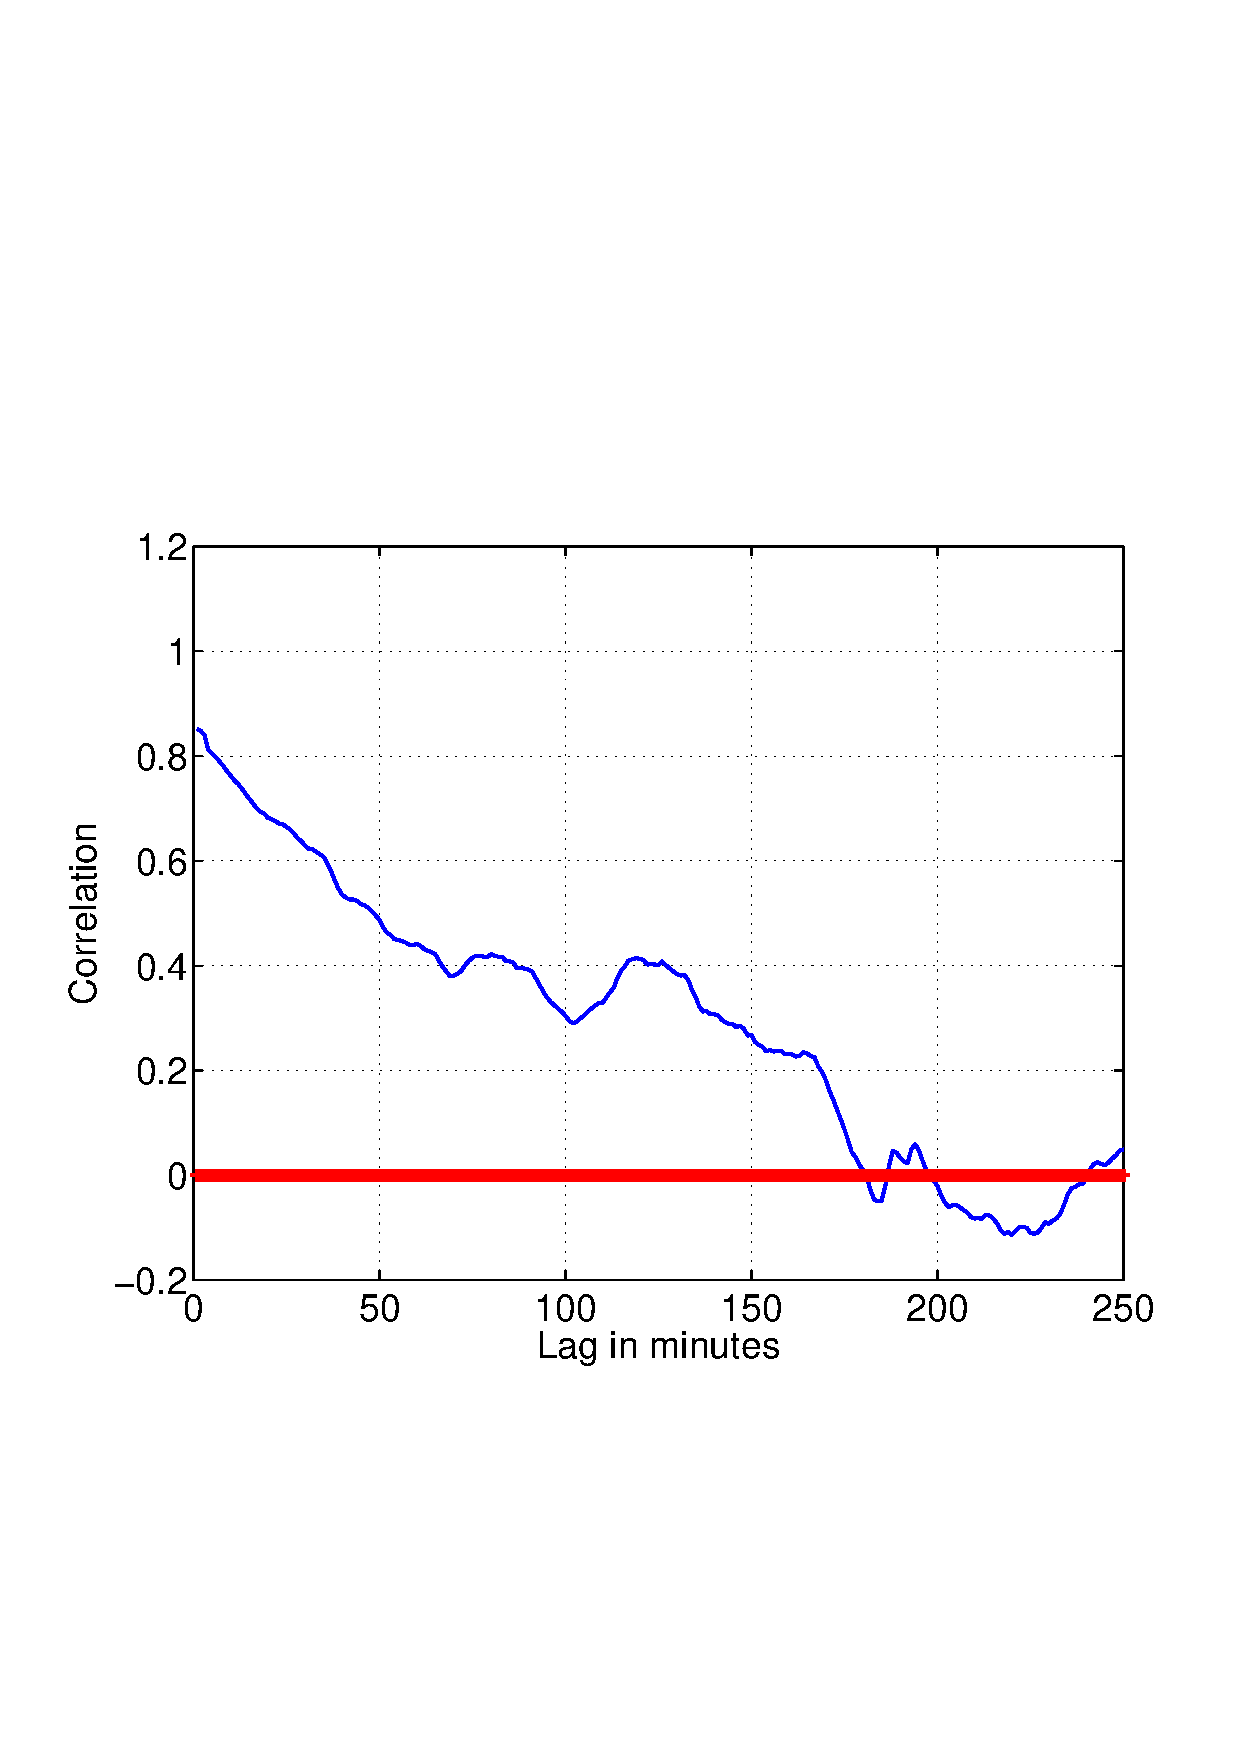
\includegraphics[scale=0.50]{{Figures/GIClags.png}}
\caption{Correlation vs lags}
\label{Lags}
\end{figure}

Figure \ref{Lags} shows a set of predictions made for autocorrelation in geomagnetically-induced currents (GIC). This metric is a measure of how much electric currents in the magnetosphere induce currents in ground-based electrical systems. The predictions were made further and further in time from the current magnetic field and GIC measurements, with decreasing accuracy as the predicted time got further from the current time. While an accurate prediction can be made one minute in advance, a prediction 3 hours in advance has almost no correlation with what actually happens. This is the main problem that this dissertation hopes to address.


\subsection{Nonlinear approaches}
Other models will be devised to test nonlinear approaches to forecasting. One common choice are models based on neural networks \cite{NNARMA,ANNforecast} which allow for a model that can approximate a non-linear system. The usefulness of this is apparent in a few key points: the weights of contribution of any particular variable to a system will likely be nonlinear in some fashion (e.g. a ground station's measurements will depend on sunlight heating the ionosphere which depends on latitude, time of year, and time of day), and allowing for the non-linear effects of saturation where perhaps the magnetosphere will behave differently after reaching certain levels of particle density or electric potential.

Another algorithm known as Principal Component Analysis (PCA) can be used to take the large number of possible variables and define an orthogonal set of vectors that most efficiently encapsulate the variance in the data. By doing this, the number of variables needed for computing any linear or non-linear algorithm can be reduced and optimized, making predictions quicker while maintaining most of the predictive benefits of using all possible data.




\chapter[Models]{Models}

\section{ARMAX}

\subsection{Overview}

\subsection{Applicability}

\subsection{Caveats and Biases}

\subsection{Mean vs Median}

\subsection{Effects of time averaging}

\subsection{Results and Analysis}



\section{Neural Net}

\subsection{Overview}

\subsection{Applicability}

\subsection{Caveats and Biases}

\subsection{Parameters and Inputs}

\subsection{Results and Analysis}

\subsection{Comparison to Linear Model}

\section{Hybrid?}

%% Note: appendix is now put before bibliography.
%% include the following directives if there are any appendices
\appendix
\appendixeqnumbering
\include{Appendix}

%%
%%  bibliography
%%

%% list all of the BibTeX files here for the WinEdt project (if applicable)
%GATHER{bibfile.bib}

%% any bibliography style can be used, but IEEEtran.bst is ideally suited to
%% electrical engineering references

\bibliographystyle{IEEEtran}
\bibliography{bibfile}

%%
%% curriculum vitae
%%
\cvpage

\noindent Include your \emph{curriculum vitae} here detailing your background,
education, and professional experience.
\end{document}
